\documentclass[letterpaper,10pt]{article}
\usepackage[top=2cm, bottom=1.5cm, left=1cm, right=1cm]{geometry}
\usepackage{amsmath, amssymb, amsthm,graphicx, enumitem}
\usepackage{fancyhdr}
\pagestyle{fancy}
\lhead{\today}
\chead{MSCS 791 Mayo Project Proposal and Timeline}
\rhead{Justin Hood}
\newcommand{\Z}{\mathbb{Z}}
\newcommand{\Q}{\mathbb{Q}}
\newcommand{\R}{\mathbb{R}}
\newcommand{\C}{\mathbb{C}}
\newtheorem{lem}{Lemma}
\begin{document}
In this case study, we are tasked with optimizing a pharmacies workflow under the constraints related to both the number of and types of employees available.\\\\
The initial problem that must be solved is to construct a model of the starting conditions. We are given that there are 5 pharmacy technicians and 2 pharmacists available to work in our hypothetical pharmacy environment, wherein they process two types of drugs, oral and IV. These two different jobs have tasks as follows:
\begin{center}
\begin{tabular}{|c|c|}
\hline
Technician & Pharmacist\\\hline\hline
Order Entry & Order Entry \\\hline
& Entry Verification \\\hline
Drug Preparation & Drug Preparation\\\hline
& Preparation Verification\\\hline
Distribution through Window & Distribution through Window\\\hline
\end{tabular}
\end{center}
So, we see that the tasks that a technician may perform are a proper subset of the tasks a pharmacist may perform. In addition to this role constraint, only one technician is initially allocated to the task of filling IV specific prescriptions. First, a full process flow chart must be constructed. Based on the rough explanation in the problem and an initial study of the given papers, we may construct an initial flowchart as follows:
\begin{center}
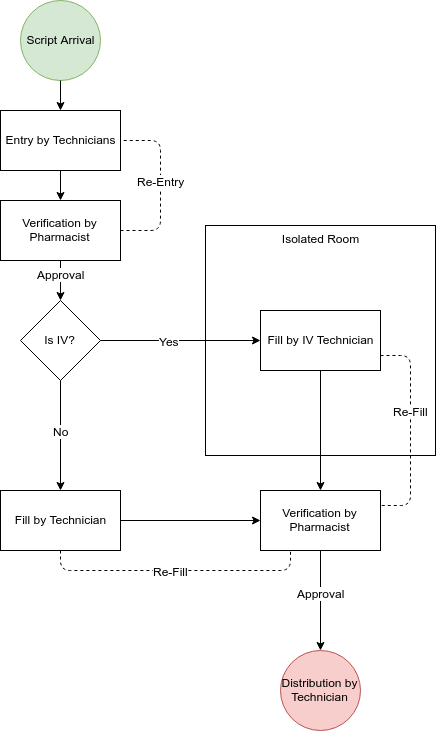
\includegraphics[scale=.5]{Flowchart.png}
\end{center}
We note that in our rough chart, that the filling of the IV prescription is done in an isolated room by an individual technician, which will present a challenge when it comes to the construction of the model.\\\\
In addition to the working constraints, we are also provided with data related to the incoming order times for both IV and oral drugs. We know that the IV times are distributed exponentially, but the oral distribution is unknown. In order to model this pharmacy environment, the distribution of this data set must be identified. If I recall correctly we may be able to compare the unknown data to other potential distributions using the Kolmogorov-Smirnov test. This test will enable us to compare the data to potential distributions, with the only weakness coming from our lack of knowledge of the parameters in the potential distribution, however it is possible to rule out distributions based on the shape of the data itself, reducing the number of parameter estimates required. This same process can be applied to the data for entry, prep, and verification times.\\\\
With these distribution estimates in hand, as well as our model of the process, we can use a discrete event modeling program such as Arena to simulate the events over a day of work. Software like Arena will provide us with the necessary statistics for the problem, like utilization of employees.\\\\
Using the results from our simulation, we will attempt to optimize the process. This could involve increasing or decreasing employees in either category, as well as changing the workflow of the process dependent on the results of the summary statistics from the base model.\\\\
A tentative timeline follows:\\
\begin{itemize}
\item October 13-18: Review provided material. Establish complete understanding of problem, and ask relevant initial questions related to the parameters of the problem. Review relevant concepts for distributions, and Arena programming.
\item October 19-22: Analyze the unknown data distributions to arrive at potential models. Attempt a first run in Arena of base model.
\item October 23: Status Report \# 1
\item October 24-31: Refine model in Arena. Ensure base case is correct.
\item November 1-7: Consider potential optimizations to the model, begin implementation.
\item November 8-13: Fully implement optimizations in model, address any issues that arise from comparison to base case.
\item November 13: Status Report \# 2
\item November 14-21: Begin drafting of project, construction of relevant figures and summary data sets.
\item November 22-Dec 1: Finish Draft
\item December 2: Rough Draft
\item December 3-12: Use feedback to correct and finish project.
\item December 13: Final Project Submission
\end{itemize}
\end{document}
